\section{Track selection \label{sec:trackselection}}
Tracks are associated to jets using a cone in $\eta - \phi$ space defined as $\Delta R = \sqrt{\Delta \eta^2 + \Delta \phi^2} < 0.5$. A new development which introduces a variable cone size is discussed in Section~\ref{sec:dvelopments}. 

Furhter selection criteria for tracks are listed in the following. The corresponding distributions for all tracks within a distance $\Delta R < 0.5$ to the jet axis are displayed in Figures~\ref{fig:inputVars1} to \ref{fig:inputVars3}.
\begin{itemize}
\item number of pixel hits $>= 2$  (Figure \ref{fig:inputVars1})
\item number of tracker hits (including pixel) $>= 8$ (Figure \ref{fig:inputVars1})
\item transverse impact parameter $|IP_{2D}| < 0.2$~cm (Figure \ref{fig:inputVars1})
\item transverse momentum $p_t > 1$~GeV/$c$ (Figure \ref{fig:inputVars2})
\item normalized $\chi^2 < 5$ (Figure \ref{fig:inputVars2})
\item longitudinal impact parameter $|IP_{z}|< 17$~cm (Figure \ref{fig:inputVars2})
\item distance to jet axis $ < 0.07$~cm (Figure \ref{fig:inputVars3})
\item decay length $< 5$ (Figure \ref{fig:inputVars3})
\end{itemize}
Figures~\ref{fig:inputVars1} to \ref{fig:inputVars3} show the track selection variables without any cuts, while Figures~\ref{fig:inputVars1N} to \ref{fig:inputVars3N} show the same variables but with all cuts, except for the cut on the variable displayed ($n$-1 cuts).
\begin{figure}[h!]
\centering
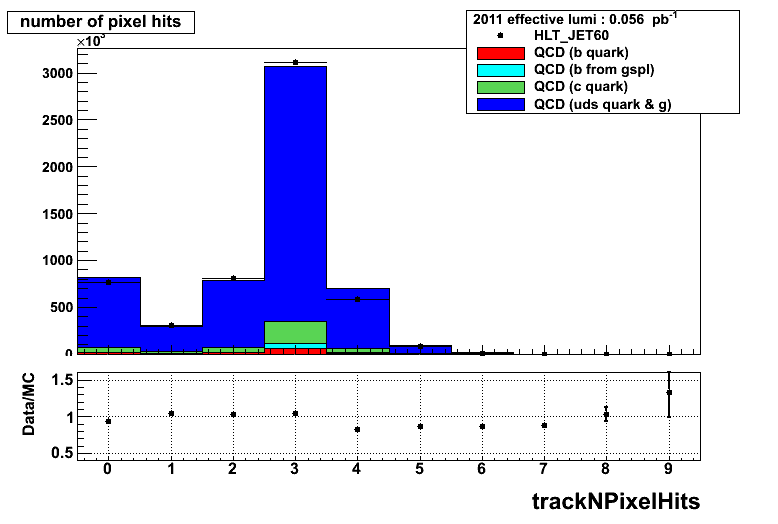
\includegraphics[width=0.32\textwidth]{figures/trackNPixelHits_Linear.png}
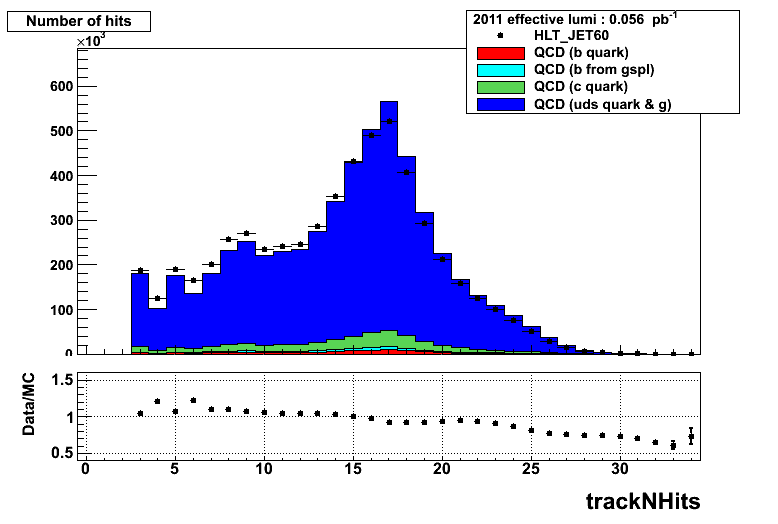
\includegraphics[width=0.32\textwidth]{figures/trackNHits_Linear.png}
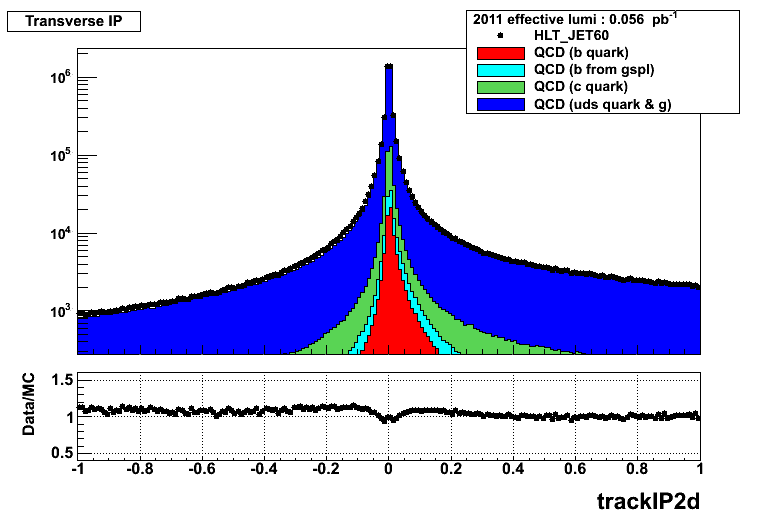
\includegraphics[width=0.32\textwidth]{figures/trackIP2d_Log.png}
\caption{Left: number of hits in the pixel detector, middle: total number of hits in the tracker, right: transverse track impact parameter. No cuts on  track variables were applied.}
\label{fig:inputVars1}
\end{figure}

\begin{figure}[h!]
\centering
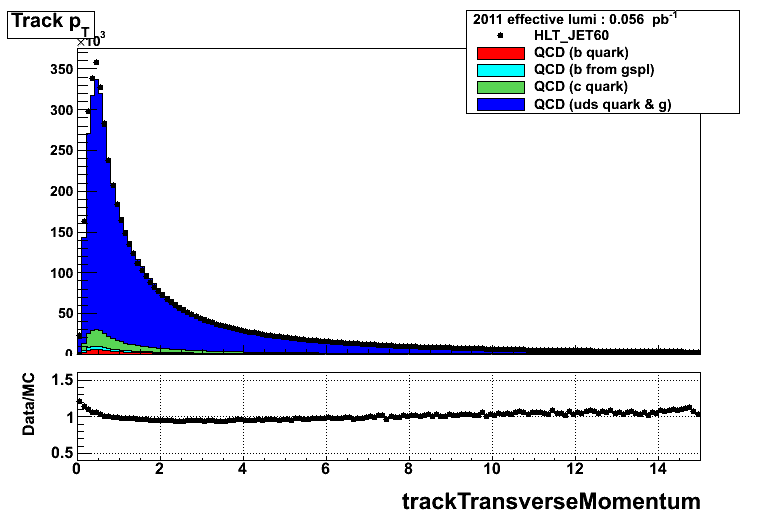
\includegraphics[width=0.32\textwidth]{figures/trackTransverseMomentum_Linear.png}
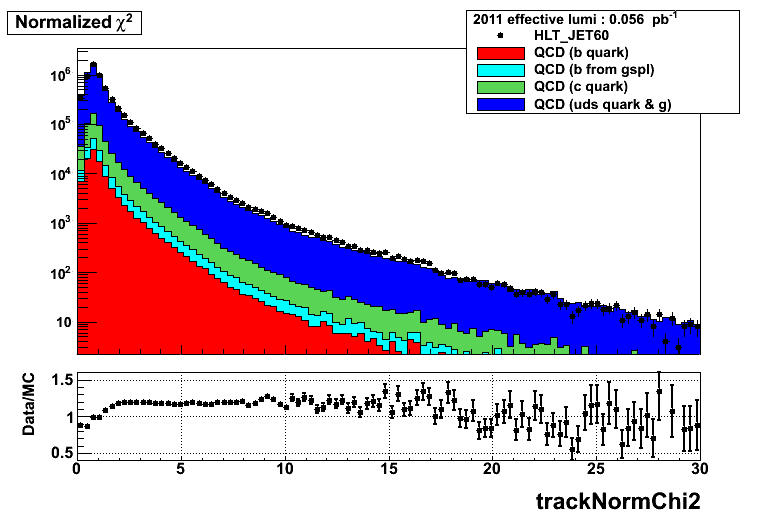
\includegraphics[width=0.32\textwidth]{figures/trackNormChi2_Log.png}
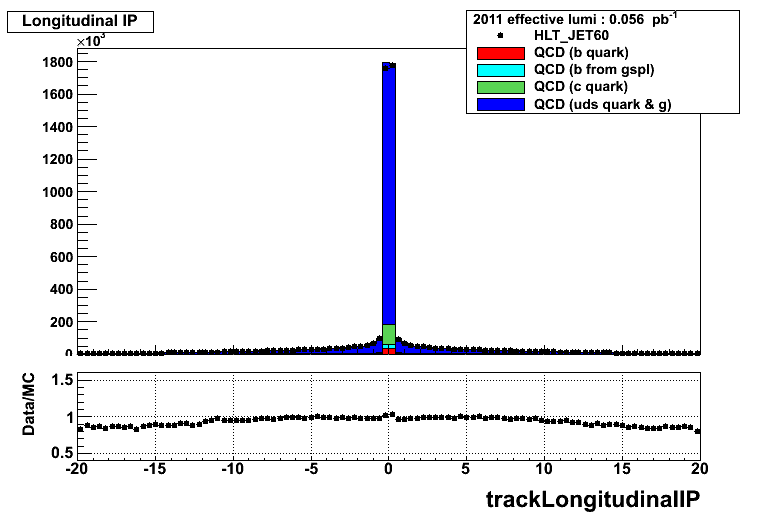
\includegraphics[width=0.32\textwidth]{figures/trackLongitudinalIP_Linear.png}
\caption{Left: transverse track momentum, middle: normalized track $\chi^2$, right: longitudinal impact parameter.  No cuts on track variables were applied.}
\label{fig:inputVars2}
\end{figure}

\begin{figure}[h!]
\centering
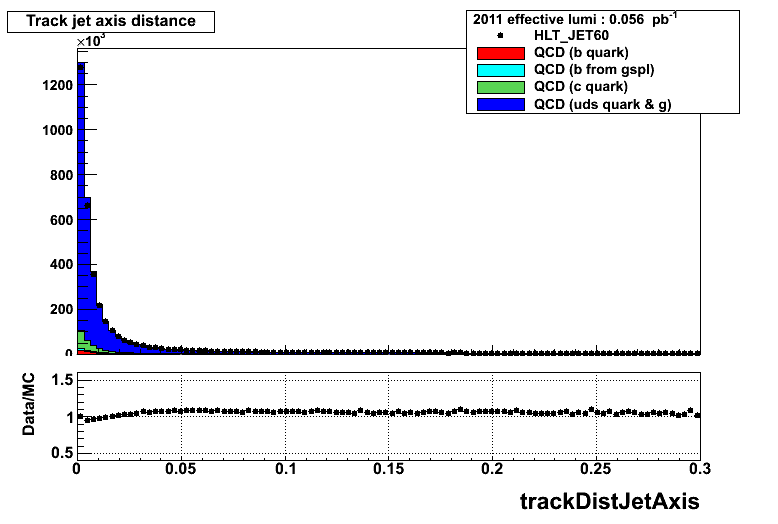
\includegraphics[width=0.42\textwidth]{figures/trackDistJetAxis_Linear.png}
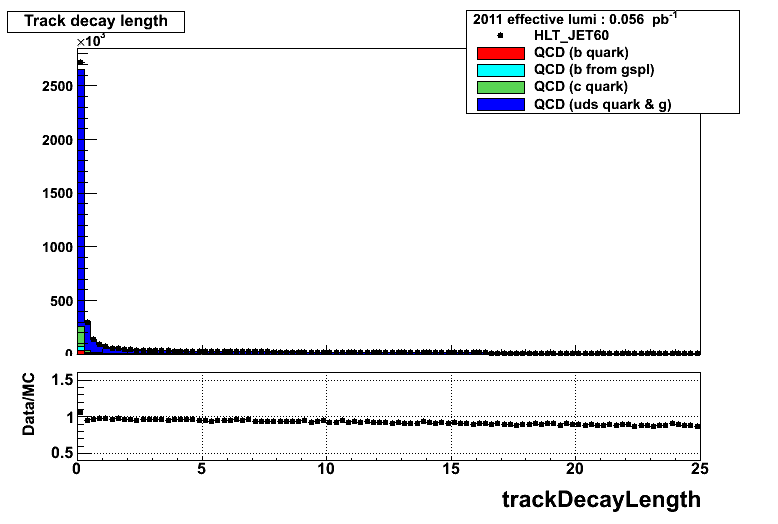
\includegraphics[width=0.42\textwidth]{figures/trackDecayLength_Linear.png}
\caption{Left: distance to jet axis, right: track decay length.  No cuts on track variables were applied. }
\label{fig:inputVars3}
\end{figure}

\begin{figure}[h!]
\centering
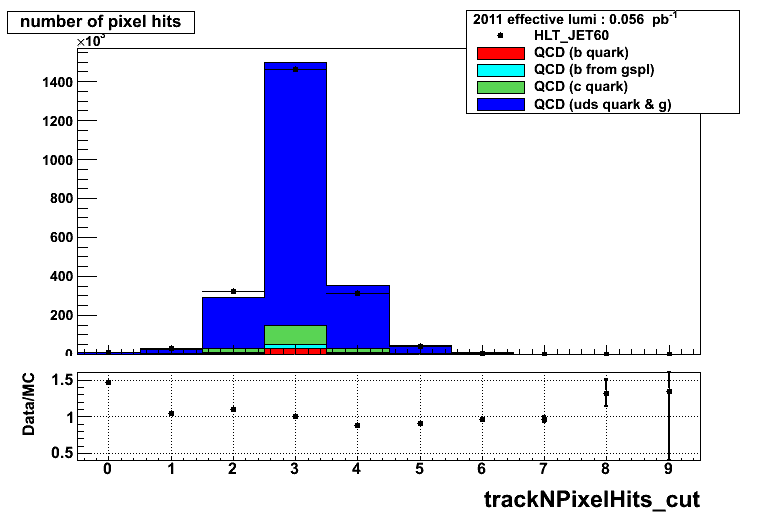
\includegraphics[width=0.32\textwidth]{figures/trackNPixelHits_cut_Linear.png}
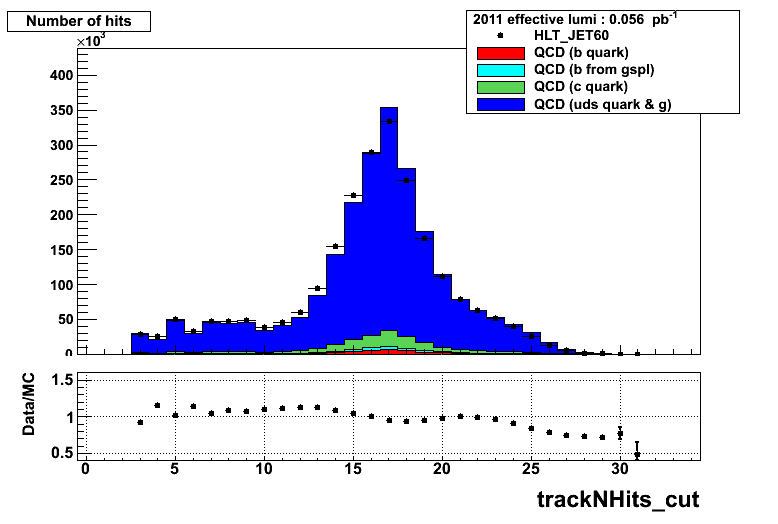
\includegraphics[width=0.32\textwidth]{figures/trackNHits_cut_Linear.png}
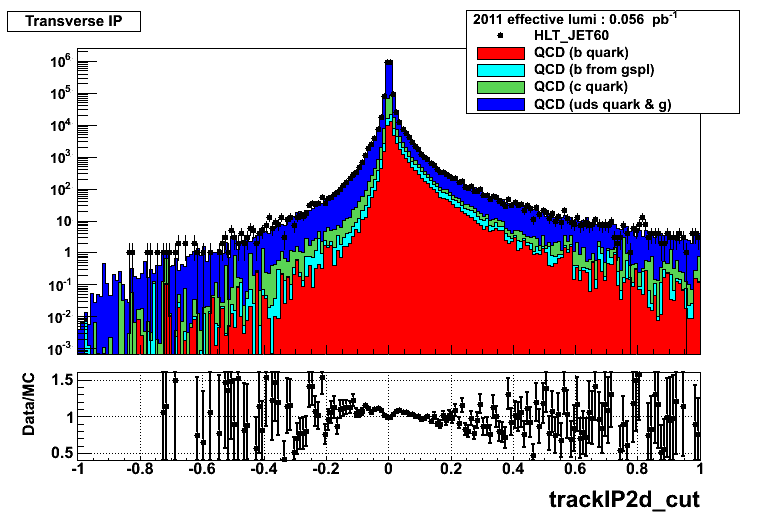
\includegraphics[width=0.32\textwidth]{figures/trackIP2d_cut_Log.png}
\caption{Left: number of hits in the pixel detector, middle: total number of hits in the tracker, right: transverse track impact parameter.  All cuts on track selection variables were applied, except for the cut on the displayed quantity.}
\label{fig:inputVars1N}
\end{figure}

\begin{figure}[h!]
\centering
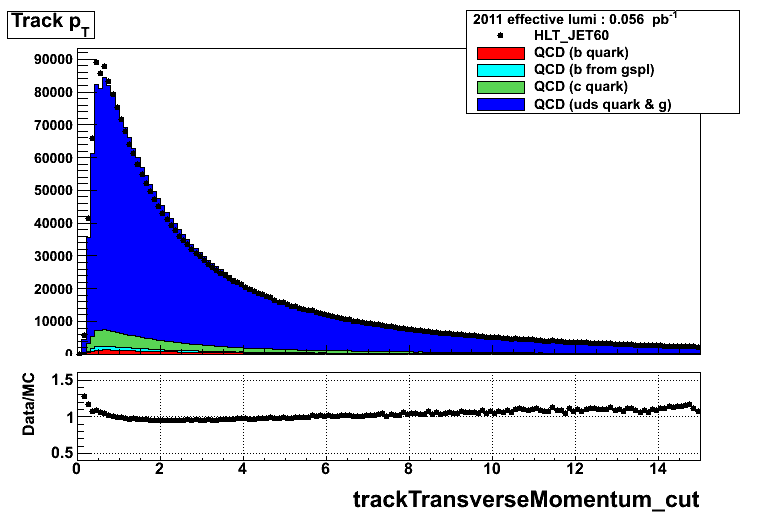
\includegraphics[width=0.32\textwidth]{figures/trackTransverseMomentum_cut_Linear.png}
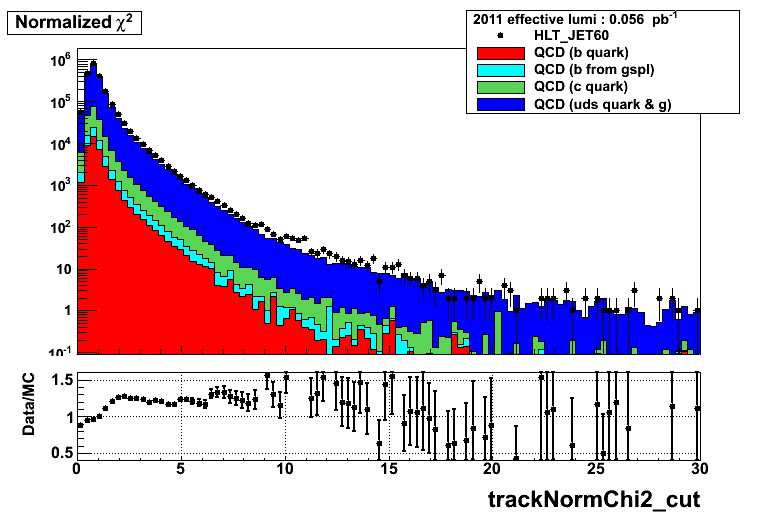
\includegraphics[width=0.32\textwidth]{figures/trackNormChi2_cut_Log.png}
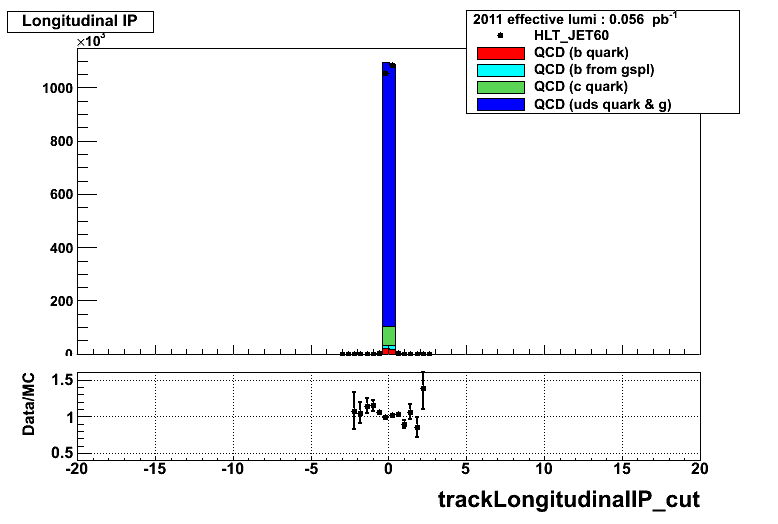
\includegraphics[width=0.32\textwidth]{figures/trackLongitudinalIP_cut_Linear.png}
\caption{Left: transverse track momentum, middle: normalized track $\chi^2$, right: longitudinal impact parameter.   All cuts on track selection variables were applied, except for the cut on the displayed quantity.}
\label{fig:inputVars2N}
\end{figure}

\begin{figure}[h!]
\centering
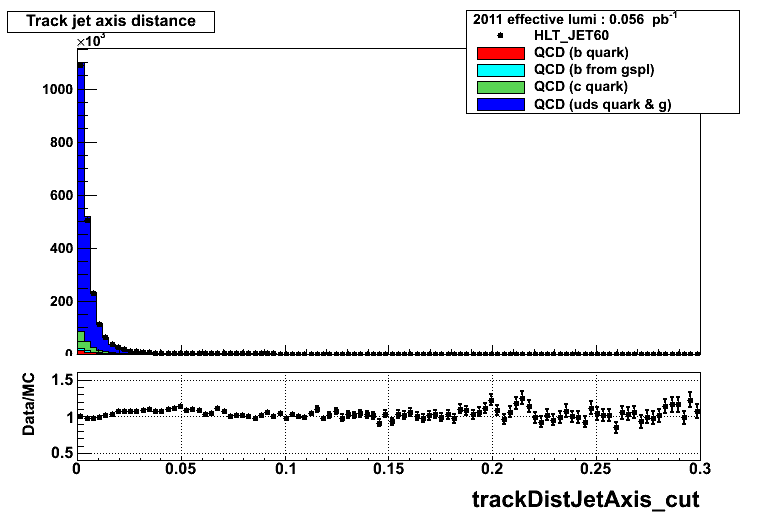
\includegraphics[width=0.42\textwidth]{figures/trackDistJetAxis_cut_Linear.png}
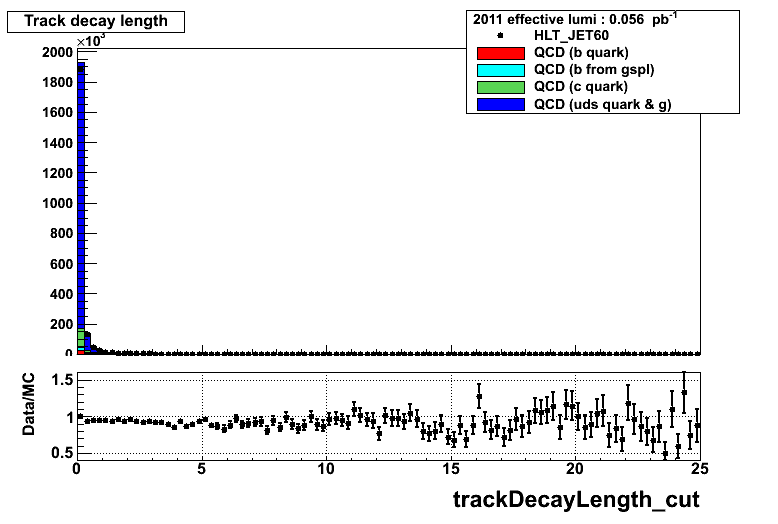
\includegraphics[width=0.42\textwidth]{figures/trackDecayLength_cut_Linear.png}
\caption{Left: distance to jet axis, right: track decay length.  All cuts on track selection variables were applied, except for the cut on the displayed quantity. }
\label{fig:inputVars3N}
\end{figure}



This track selection is used for all impact parameter based algorithms, i.e. the track counting and track probability algorithms. The secondary vertex based algorithms apply slightly different selection criteria (only those which are different are listed in the following):
\begin{itemize}
\item jet-track association cone $\Delta R < 0.3$
\item distance to jet axis $ < 0.2$~cm
\item no cut on decay length
\item track quality class = "high purity" 
\end{itemize}

The average number of tracks per jet is displayed in Figure~\ref{fig:trackMult} 
for the case with and without track selection cuts.  The average number of tracks also depends on the jet energy which is shown in Figure~\ref{fig:trackMultVsPt}. The discrepancy between data and simulation is attributed to the Monte Carlo event generator which is not reproducing the charged particle kinematics perfectly.


\begin{figure}[h!]
\centering
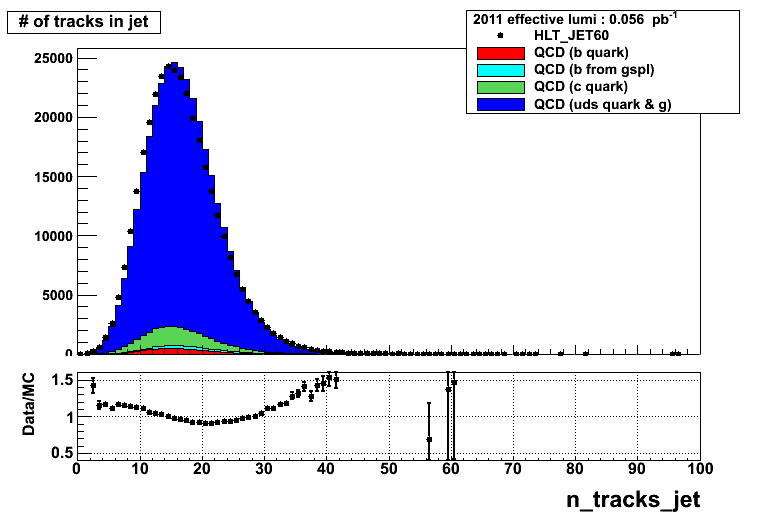
\includegraphics[width=0.42\textwidth]{figures/n_tracks_jet_Linear.png}
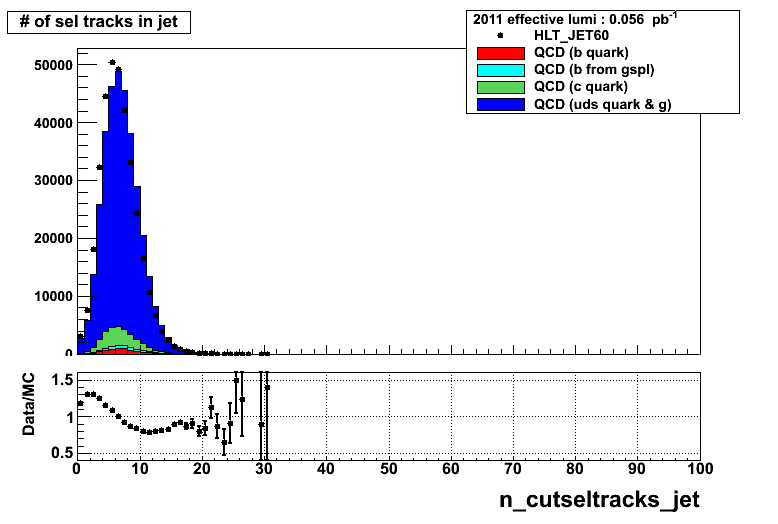
\includegraphics[width=0.42\textwidth]{figures/n_cutseltracks_jet_Linear.png}
\caption{Left: number of tracks within $\Delta R < 0.5$ of the jet axis. Right: the same for tracks passing the selection criteria of the IP based algorithms as explained in the text.}
\label{fig:trackMult}
\end{figure}

\begin{figure}[h!]
\centering
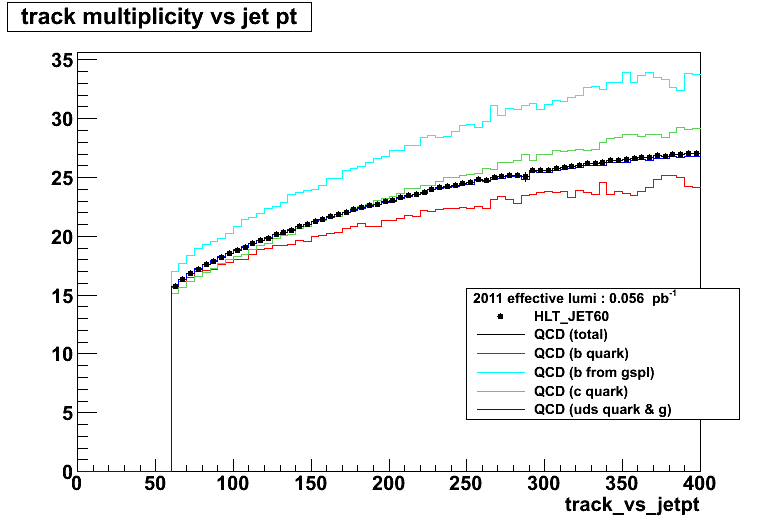
\includegraphics[width=0.42\textwidth]{figures/track_vs_jetpt_Linear.png}
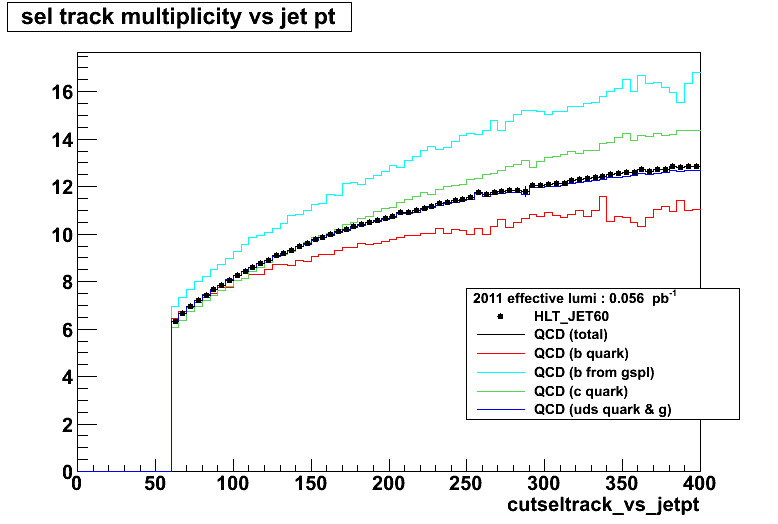
\includegraphics[width=0.42\textwidth]{figures/cutseltrack_vs_jetpt_Linear.png}
\caption{Left: average number of tracks associated to a jet depending on transverse jet momentum $p_t$. Right:  average number of selected tracks associated to a jet depending on transverse jet momentum $p_t$.}
\label{fig:trackMultVsPt}
\end{figure}
